\subsection{Основы геометрии Римана}

\textbf{2.1. Объем и радиус инъективности.} Одним важным общим понятием, которое 
используется в дальнейшем, является понятие того, что многообразие не схлопывается 
в какой-то точке. Пусть у нас есть точка $x$ в полном римановом $n$-мерном многообразии. 
Мы говорим, что многообразие \textit{$\kappa $-не-коллапсируемо} в точке $x$, если 
выполняется следующее условие: для любого $r$, при котором норма тензора кривизны Римана
$| Rm| $ не превышает $r^{-2}$ во всех точках метрического шара $B(x,r)$ радиуса $r$, центрированного 
в $x$, выполняется Vol$B(x,r)\geq \kappa r^{n}$. Существует связь между этим понятием и радиусом 
инъективности многообразия $M$ в точке $x$. А именно, если $| Rm| \leq r^{-2}$ на $B(x,r)$ и если 
$B(x,r)$ \textit{$\kappa $-не-коллапсируемо}, то радиус инъективности многообразия $M$ в точке 
$x$ больше или равен положительной константе, которая зависит только от $r$ и $\kappa $. 
Преимущество работы с условием объема, не приводящим к схлопыванию, заключается в том, 
что, в отличие от радиуса инъективности, существует простое уравнение для эволюции объема 
под действием потока Риччи.

Еще одним важным общим результатом является теорема о сравнении объемов Бишопа-Громова, 
которая утверждает, что если кривизна Риччи полного риманова $n$-мерного многообразия $M$ 
ограничена снизу постоянной $(n-1)K$, то для любой точки $x\in M$ отношение объема шара 
$B(x,r)$ к объему шара радиуса $r$ в пространстве постоянной кривизны $K$ является 
невозрастающей функцией, предел которой при $r\rightarrow 0$ равен $1$. 

Все эти базовые факты из римановой геометрии рассматриваются в первой главе.\\


\textbf{2.2. Многообразия с неотрицательной кривизной.} По причинам, которые должны стать 
ясными из вышеизложенного и, в любом случае, станут еще более очевидными вскоре, 
многообразия с неотрицательной кривизной играют чрезвычайно важную роль в анализе 
потоков Риччи с хирургией. Нам нужно несколько общих результатов о них. 
Первый — это теорема о душе для многообразий с неотрицательной секционной кривизной. 
\textit{Душа} — это компактное, тотально геодезическое подмногообразие. Все многообразие 
диффеоморфно полному пространству векторного расслоения над любой из своих душ. 
Если некомпактное $n$-мерное многообразие имеет положительную секционную кривизну, 
то любая душа для него — это точка, и, в частности, это многообразие диффеоморфно 
евклидову пространству. Кроме того, функция расстояния $f$ от души имеет свойство, 
что для каждого $t > 0$ прообраз $f^{-1} (t)$ гомеоморфен ($n-1$)-сфере, а прообраз под 
этой функцией расстояния любого недегенерированного интервала $I\subset \mathbb{R}^{+}$ гомеоморфен 
$S^{n-1} \times I$.

Другим важным результатом является теорема о расщеплении, которая гласит, что если полное 
многообразие неотрицательной кривизны в сечении имеет геодезическую линию (изометрическую копию 
$\mathbb{R}$), расстояние между каждой парой его точек которой минимизировано, то это многообразие 
является метрическим произведением многообразия на одну меньшую размерность и $\mathbb{R}$. В частности, если 
полное $n$-многообразие неотрицательной секционной кривизны имеет два конца, то это 
метрическое произведение $N^{n-1} \times \mathbb{R}$, где $N^{n-1}$ — компактное многообразие.

Кроме того, нам нужны некоторые элементарные результаты сравнения из теории Топоногова. 
В них сравниваются обычные треугольники на евклидовой плоскости с треугольниками в многообразии 
неотрицательной кривизны в разрезе, стороны которых минимизируют геодезические в этом 
многообразии.\\

\textbf{2.3. Канонические окрестности.} Большая часть анализа геометрии потоков Риччи связана 
с понятием канонических окрестностей. Зафиксируем некоторое достаточно малое значение 
$\epsilon > 0$. Существует два типа некомпактных канонических окрестностей: $\epsilon$-шейки и $\epsilon$-шапки.
В римановом 3-многообразии $(M,g)$ $\epsilon$-шея, центрированная в точке $x\in M$, — это подмногообразие 
$N\subset M$ и диффеоморфизм $\psi:S^{2} \times (-{\epsilon}^{-1} ,{\epsilon}^{-1})\rightarrow N$, 
такие что $x\in \psi(S^{2} \times \{0\})$, а также такие, 
что обратный образ масштабированной метрики $\psi^{*} (R(x)g)$ отличается от произведения 
стандартной метрики с кривизной $1$ на $S^{2}$ и обычной метрики на интервале $(-{\epsilon}^{-1} ,{\epsilon}^{-1})$ 
не более чем на $\epsilon$ в $C^{[1/\epsilon]}$-топологии. (Здесь $R(x)$ обозначает скалярную кривизну 
$(M,g)$ в точке $x$).
$\epsilon$-шапка — это некомпактное подмногообразие $\mathcal{C} \subset M$, обладающее свойством того, что 
некоторая окрестность бесконечности $N$ в $\mathcal{C}$ является $\epsilon$-шеей, а так же свойством того, что 
каждая точка $N$ является центром $\epsilon$-шеи в $M$ и что 
\textit{ядро} $\mathcal{C} \setminus \overline{N}$ $\epsilon$-шапки диффеоморфно либо 3-шару, либо проколотой $\mathbb{RP}^3$.
Также важно рассматривать $\epsilon$-шапки, которые после масштабирования 
(чтобы $R(x)=1$ для некоторой точки $x$ в шапке) обладают ограниченной 
геометрией (ограниченный диаметр, ограниченное соотношение кривизн 
в любых двух точках и ограниченный объём). Если $C$ задаёт границу 
для этих величин, то такую шапку называют $(C,\epsilon)$-шапкой (см. \textsc{Рис.} \ref{fig:fig1}).
$\epsilon$-трубка в $M$ — это подмногообразие $M$, диффеоморфное $S^{2}\times (0,1)$, 
являющееся объединением $\epsilon$-шеек и обладающее свойством, что каждая 
точка $\epsilon$-трубки является центром $\epsilon$-шеи в $M$.
\begin{figure}[h]
    \centering
    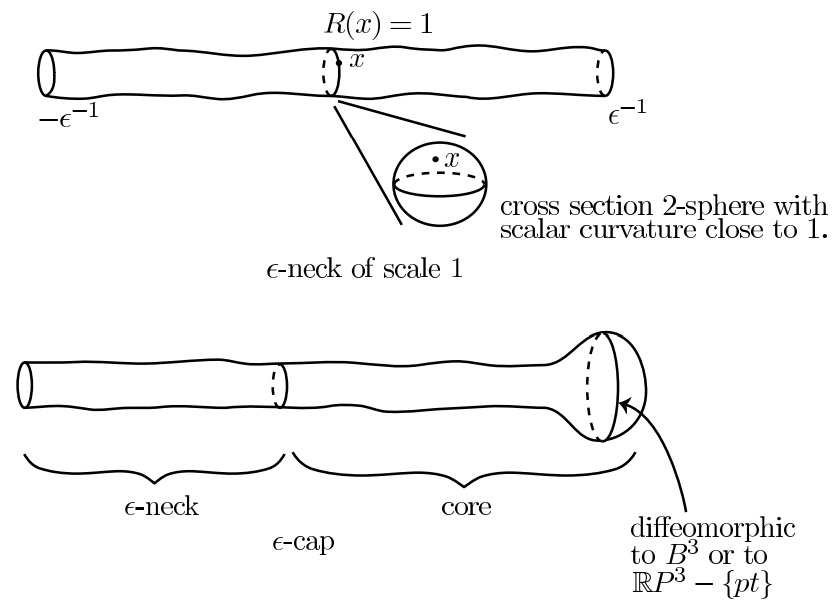
\includegraphics[width=\textwidth]{chapterIntro/subsection2/1.jpg}
    \caption{Канонические окрестности.}
    \label{fig:fig1}
\end{figure}

Существует два других типа канонических окрестностей в $3$-многообразиях: 
(i) $C$-компонента и (ii) $\epsilon$-круглая компонента. $C$-компонента — это компактное 
связное риманово многообразие с положительной секционной кривизной, 
диффеоморфное либо $S^{3}$, либо $\mathbb{RP}^3$, с тем свойством, что масштабирование 
метрики с использованием $R(x)$ для любой точки $x$ в компоненте приводит к 
римановому многообразию, диаметр которого не превышает $C$, секционная 
кривизна в любой точке и в любом направлении $2$-плоскости находится между 
$C^{-1}$ и $C$, а объём находится между $C^{-1}$ и $C$. 
$\epsilon$-круглая компонента — это компонента, на которой метрика, масштабированная 
с использованием $R(x)$ для любой точки $x$ в компоненте, находится в пределах 
$\epsilon$ в $C^{[1/\epsilon]}$-топологии от круглой метрики с скалярной кривизной, 
равной единице.

Как мы увидим, сингулярности на момент времени $T$ трехмерного 
потока Риччи содержатся в подмножествах, которые являются 
объединениями канонических окрестностей относительно метрик 
на более ранних моментах времени $t^{\prime } <T$. Таким образом, нам 
нужно понять топологию многообразий, которые являются 
объединениями $\epsilon$-трубок и $\epsilon$-шапок. Основное наблюдение состоит 
в том, что, при условии, что $\epsilon$ достаточно мало, когда две 
$\epsilon$-шейки пересекаются (в более чем небольшой окрестности их 
границ), их произведенные структуры почти выравниваются, так 
что две $\epsilon$-шейки можно склеить вместе, чтобы образовать 
многообразие, волоконированное $S^2$ -связкой над $S^1$. 
Этот топологический результат доказан в приложении в конце 
книги. Мы зафиксируем $\epsilon >0$, достаточно малое, чтобы эти 
результаты выполнялись. Используя эту идею, мы показываем, 
что для $\epsilon >0$, достаточно малого, если связное многообразие 
является объединением $\epsilon$-трубок и $\epsilon$-шапок, то оно 
диффеоморфно одному из следующих: $\mathbb{R}^3$, 
$S^2 \times \mathbb{R}$, $S^3$, $S^2 \times S^1$, $\mathbb{RP}^3 \#\mathbb{RP}^3$, 
полное пространство линейного расслоения над 
$\mathbb{RP}^2$ или неориентируемое $2$-сферическое расслоение над 
$S^1$. Этот топологический результат доказан в приложении в конце книги. 
\textbf{Мы зафиксируем $\epsilon >0$, достаточно малое, чтобы эти результаты выполнялись.}

Существует один результат, связанный с каноническими окрестностями 
и многообразиями с положительной кривизной, который мы будем 
использовать неоднократно: любое полное $3$-мерное многообразие с 
положительной кривизной не допускает $\epsilon$-шеек с произвольно высокой 
кривизной. В частности, если $M$ — полное риманово $3$-мерное 
многообразие с тем свойством, что каждая точка с скалярной 
кривизной больше $r^{-2}_{0}$ имеет каноническую окрестность, то 
$M$ имеет ограниченную кривизну. 
Это оказывается центральным результатом и используется многократно. 

Все эти базовые факты о римановых многообразиях с неотрицательной кривизной 
изложены во второй главе.

